% !TeX spellcheck = en_US
% !TeX encoding = UTF-8
\chapter{BiBEx}\label{chap:bibex}

In this chapter, we present our unified system, BiBEx, which employs a cascade of ML models to extract both header and reference metadata from scientific publications. We will explain the design and architecture of our system (Section~\ref{sec:bibex_architecture}), providing insights into its underlying structure and functionality. Furthermore, we will introduce two user-friendly applications, BiBEx-UI and BiBEx-Model, that we developed to enable a efficient metadata extraction process.
Throughout this chapter, we will provide a comprehensive explanation of the workflow employed by BiBEx (Section~\ref{sec:bibex_workflow}). This will encompass the step-by-step process of how the system handles document segmentation, reference parsing, and author extraction.

% In this chapter we will introduce our unified system, BiBEx, comprising of a cascade of ML models to extract header and reference metadata. We will explain the design and architecture of our system (Section~\ref{sec:bibex_architecture}), and describe the two applications, we developed to enable a fast and user-friendly extraction process. We will also in detail explain the workflow of our system.

\section{BiBEx Architecture}\label{sec:bibex_architecture}
In order to maintain a clear separation between the User Interface and the business logic, we have developed two distinct applications. The first application, BiBEx-Model, is responsible for handling the computational logic, by processing and extracting relevant information from scientific articles utilizing our proposed ML models.\\
Meanwhile, the second application, BiBEx-UI, is designed to present visualizations of the extracted data to the user in a user-friendly manner.\\
While both solutions are designed as an ensemble of separated Web-Applications, BiBEx-Model can function as a standalone application. By utilizing its API, an user can time-efficiently query a large set of scientific literature for metadata extraction.\\
When combined, these two applications form our proposed unified Application: BiBEx.

\subsection{BiBEx-UI}\label{sec:bibex_ui}

BiBEx-UI is a user-friendly web application implemented using Vue.js~\cite{vuejs} and designed to simplify the extraction of metadata from articles for its users. It accepts input in various formats, including PDFs, scans, and raw reference text. The primary objective of BiBEx-UI is to enhance the user experience by offering an intuitive, simple, and easy-to-use interface.\\
The application further communicates with the BiBEx-Model REST API to process the input data and extract the relevant metadata. It handles all asynchronous data transfers and ensures smooth communication between the user interface and the model application.\\
In addition to its data processing capabilities, BiBEx-UI functions as visualization tool to present the results of the metadata extraction.
\newpage

\begin{figure}[!ht]
	\centering
	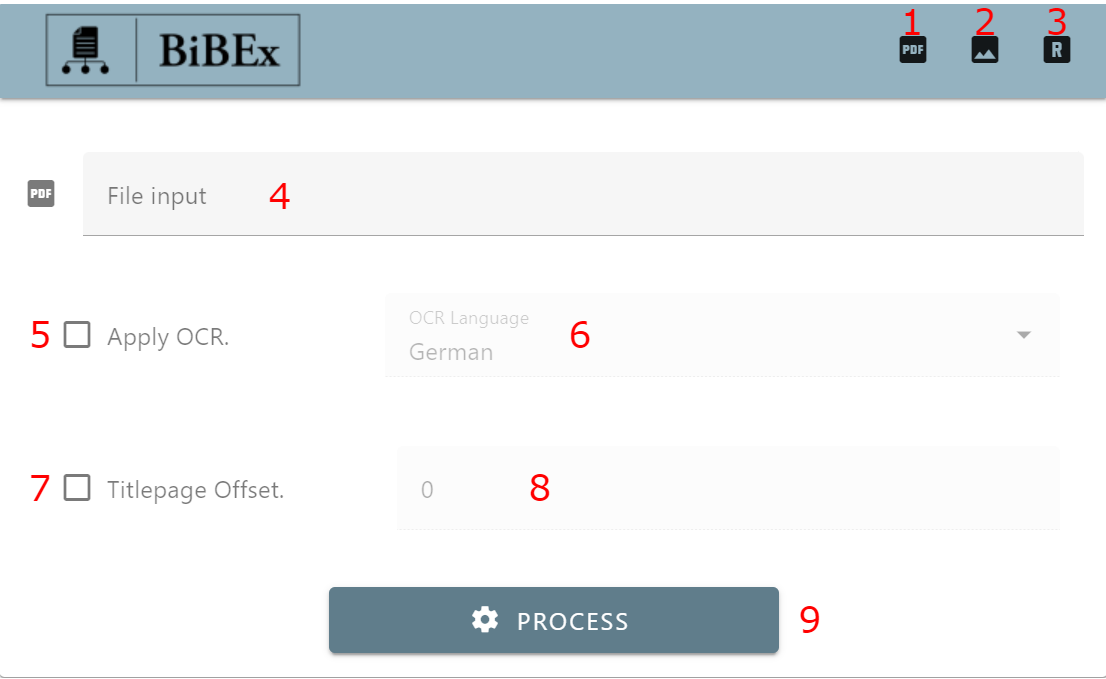
\includegraphics[width=1.0\linewidth]{images/bibex_ui.png}
	\caption{The BiBEx-UI Application provides users the capability to process their data in various forms.}
	\label{fig:bibex_ui}
\end{figure}

Figure~\ref{fig:bibex_ui} presents an exemplary overview of the User Interface for PDF data input. The UI consists of the following elements:
\begin{itemize}
    \item \textbf{[1-3]}: Mode Navigation, where an user can select between the preferred input methods as PDF \textbf{[1]}, image \textbf{[2]}, or raw reference text \textbf{[3]}.
    \item \textbf{[4]}: File Input, where the user can select a PDF file.
    \item \textbf{[5-6]}: OCR module, where the user can decide if OCR should be applied \textbf{[5]} to a PDF file and choose the language \textbf{[6]}.
    \item \textbf{[7-8]}: Titlepage offset, where an user can change the page, if desired \textbf{[7]}, which the BiBEx will use as header page \textbf{[8]}.
    \item \textbf{[9]}: Process button, where the user can start the metadata extraction process \textbf{[9]}.
\end{itemize}
\newpage

After the user clicks the \textit{Process} button, an asynchronous request is sent to the BiBEx-Model application. Subsequently, the user is redirected to a result page or, in case of unexpected behaviour, will get a dialog with an error message. The result page visualizes all relevant entities of the header extraction and the reference extraction. Moreover, users have the option to download the displayed data for their convenience. Figure~\ref{fig:bibex_output} shows a successful extraction response, visualized by the BiBEx-UI.

\begin{figure}[!ht]
	\centering
	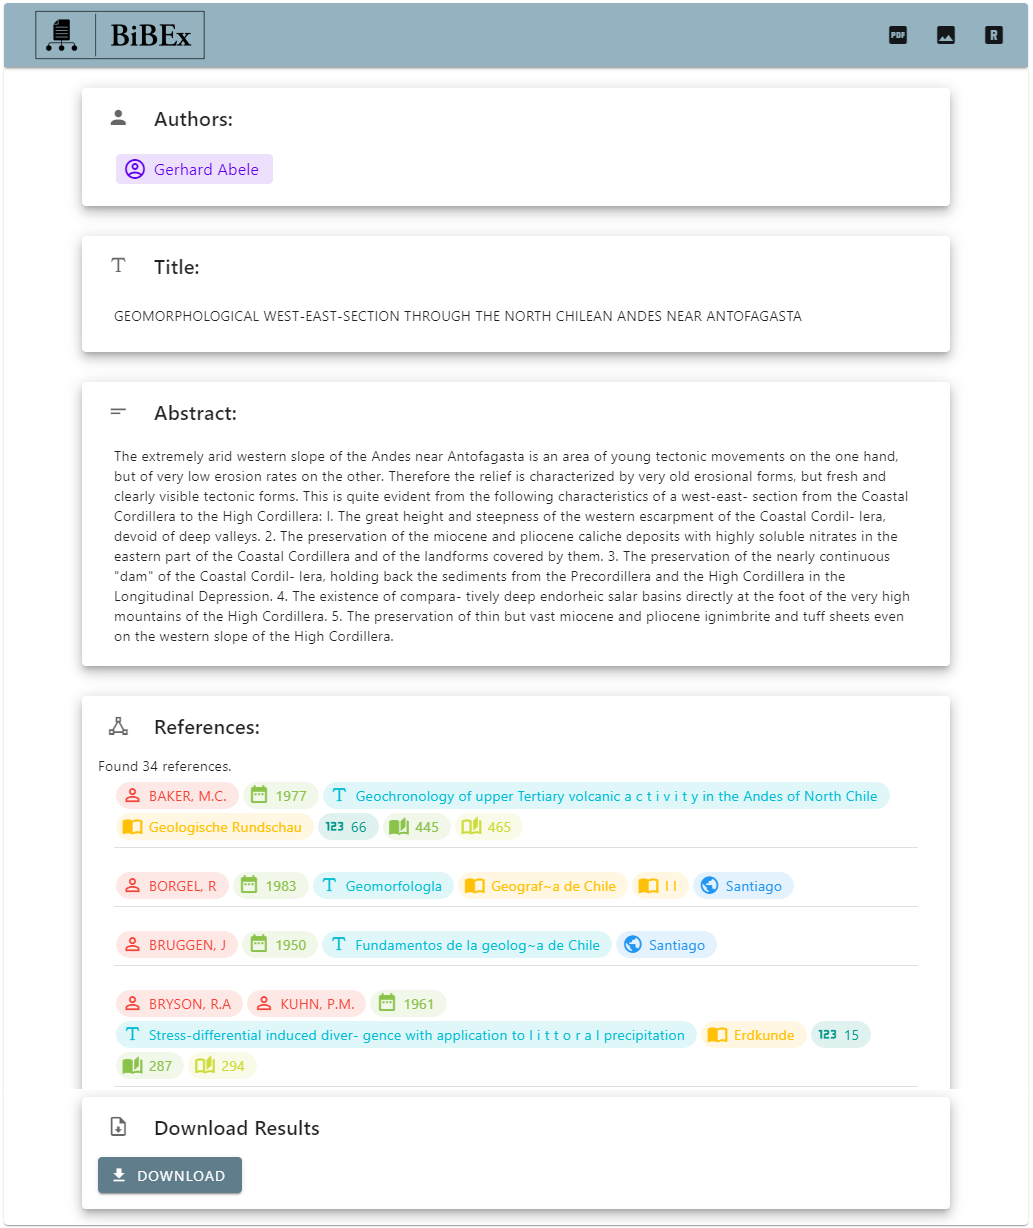
\includegraphics[width=0.7\linewidth]{images/bibex_output.png}
	\caption{The resulting output of a successful extraction process, showcased in the BiBEx-UI application.}
	\label{fig:bibex_output}
\end{figure}

\subsection{BiBEx-Model}

At its core, BiBEx-Model serves as a web application that manages the data and logic involved in the metadata extraction process. It can operate as a standalone application, allowing users to utilize its capabilities independently from BiBEx-UI, enabling swift processing of articles.\\
The application provides a REST API, developed using the FastAPI framework~\cite{fastapi}, offering three distinct endpoints resembling the different input methods.

\section{BiBEx Workflow}\label{sec:bibex_workflow}
In this section we will explain the detailed workflow of the BiBEx system, how our component models are utilized and differ during inference, and how we extract the desired metadata from publications. To offer a comprehensive understanding, we will explore all relevant system components showcased in Figure~\ref{fig:bibex_workflow}, highlighting their roles and interactions within the system.

\begin{figure}[!ht]
	\centering
	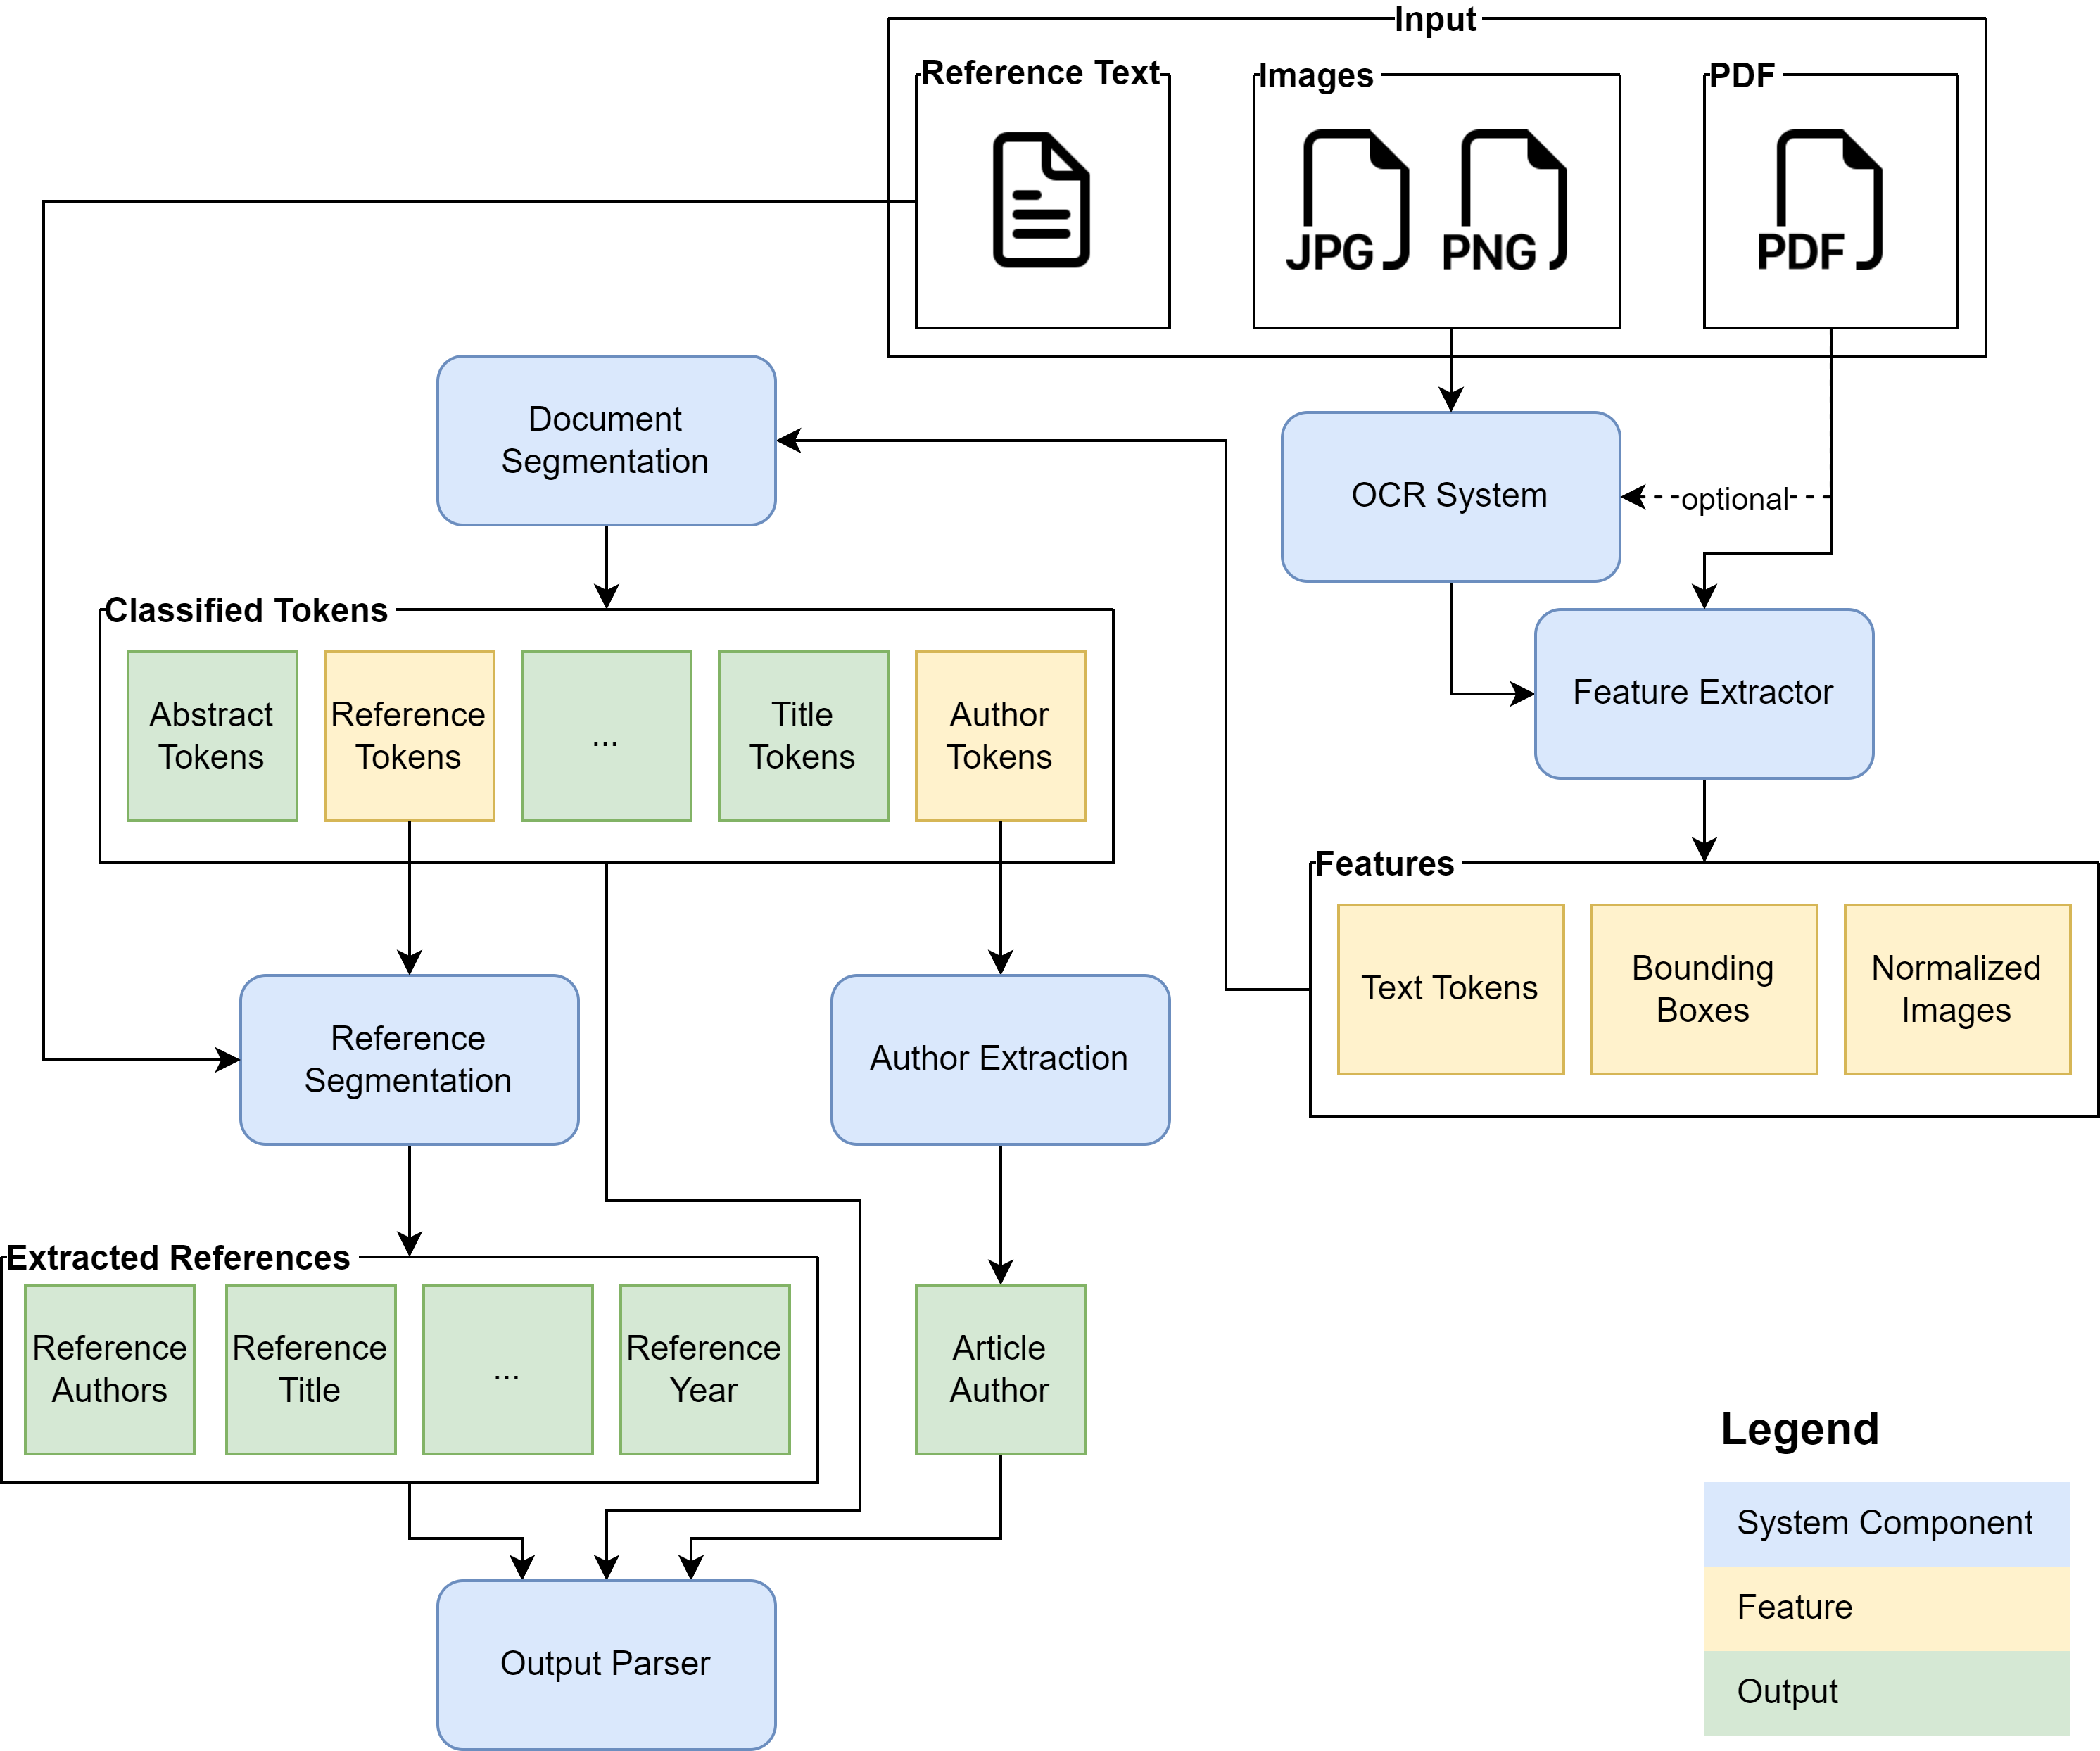
\includegraphics[width=0.7\linewidth]{images/bibex_architecture.png}
	\caption{An conceptual overview of the BiBEx workflow.}
	\label{fig:bibex_workflow}
\end{figure}

\subsection{Data Input}
As described in Section~\ref{sec:bibex_ui}, BiBEx accepts three different ways to input data as user, as PDF, PNG/JPEG images, and as plain text.

\subsection{OCR System}
We utilize the pytesseract~\cite{pytess} Python wrapper of the Tesseract Open Source OCR Engine~\cite{tesseract} to extract text from scanned images. For PDF files, this extraction step is optional, as long as the uploaded file contains a valid text layer. Furthermore, users have the flexibility to choose between English, German, French, and Spanish Tesseract language models, depending on the predominant language used in the scientific publication being processed.
\subsection{Feature Extractor}\label{sec:bibex_feature}
This System Component is responsible for further preprocessing the data and extracting features for the Document Segmentation model. As the first step, it generates normalized BGR images of all pages, ensuring consistent color representation and reducing variations across different documents. These images are resized to a standardized dimension of 224x224 pixels, resulting in a tensor shape of $(b,c,x,y)$, where $b$ denotes the batch size, $c$ the number of channels with $c=3$, $x$ the width, and $y$ the height of an image with $x=y=224$.\\
Next, we extract all word tokens and the corresponding bounding box of each token. We use the same pretrained SentencePiece tokenizer, as during our model training, which has a maximum sequence length of 512 token. In case the sequence length is below this maximum, we pad it to reach the maximum input length required by the model. Conversely, if the sequence length exceeds the tokenizer's maximum allowed length, we truncate the exceeding token.\\
Any overflowing token sequence is tokenized following the same process. The difference between the fine-tuning of our model and inference is, that we use a stride parameter of 32 token on the overflowing token to provide additional context from the previous sequence for subsequent token sequences.\\
The resulting feature set consists of tensors for input ids and attention mask, both with a dimension of $(p, b, s)$, denoting the number of pages in a transmitted article $p$, the batch size $b$, and the sequence length $s$. Additionally, bounding boxes are incorporated with a shape of $(p, b, s, 4)$, providing spatial information. Complementing these is the image tensor, which has a shape of $(p, b, c, x, y)$. Here, $p$ represents the number of pages, $b$ signifies the batch size, $c$ represents the number of image channels (set to 3), and $x$ and $y$ correspond to the width and height, respectively, of the image, both measuring 224 pixel.\\
For text layer extraction from PDFs we are using the Python package PyMuPDF~\cite{pymupdf}. For image extraction from PDF files and image conversions we utilize Pillow~\cite{clark2015pillow}.

\subsection{Document Segmentation}\label{sec:bibex_doc_seg}
The resulting batch encodings are then passed through our Document Segmentation Model, which is our fine-tuned LayoutXLM model.\\
To facilitate further processing, the model output is flattened, transforming the hierarchical representation into a sequential format. Subword token and corresponding inferred class-labels are transformed back to word-level token and labels, to pass relevant token forward to their next processing models.\\
Since we are only interested in the labels \textit{author}, \textit{reference}, and to a lesser degree \textit{title} and \textit{abstract}, we discard all other labels. Subsequent word-level token labeled as \textit{title} and \textit{abstract} are chunked together to build coherent text blocks.

\subsection{Reference Segmentation}
During this step, we focus on segmenting and parsing all tokens that have been labeled as \textit{reference} by our Document Segmentation Model. We process these tokens even if they do not form coherent text blocks, such as in cases with alternating labels or jumps between reference blocks. The idea is to extract the relevant metadata from the identified references, regardless of their arrangement.\\
The difference between fine-tuning and the production stage is, that we also use a stride parameter of 32 token as in Section~\ref{sec:bibex_feature}, taking previous context into consideration. We further utilize the whole length of our model of 512 token and do not limit our input sequence as in the training stage.\\
We utilize our Reference Parser Model with a custom pipeline, resulting in a list of grouped parsed references with the predicted entities, the textual representation, as well as start and end indices of these entities.

\subsection{Author Extraction}
In this stage, our focus lies on extracting the authors of a document. To achieve this, we treat the input again as a sequence of pretokenized token, regardless of their arrangement. We employ our Author Parser Model to extract all authors, without utilizing the stride parameter, as the number of tokens labeled as \textit{author} is unlikely to exceed our limit of 512 tokens.\\
To extract the first name and surname of document authors, as well as authors and editors from references, we employed heuristic techniques. More specifically, we devised a method that checks for specific observed author formats using regular expressions.\\
The first expression matches names with abbreviated given names at the beginning, often encountered in references, for example \textit{M. Mustermann}
\begin{Verbatim}[fontsize=\small]
    ^(?P<first>(?:[a-zA-Z]+[.][-\s]*)+)\s+(?P<last>[\w]{2,}[-'\w\s]*)+$
\end{Verbatim}
The second expression expects the surname followed by a coma and the first name, for example \textit{Mustermann, M.}
\begin{Verbatim}[fontsize=\small]
    ^(?P<last>(?:[a-zA-Z]+[-' ])*[a-zA-Z]+),\s+(?P<first>(?:[a-zA-Z][-.\s]*)+)$
\end{Verbatim}
The last expression matches the case if we have the surname followed by the first or first two uppercase letter of the first name. We encountered this case in one of the various journals in our GEOcite corpus. An example would be \textit{Mustermann MA}
\begin{Verbatim}[fontsize=\small]
    ^(?P<last>[a-zA-Z][a-zA-Z- ]+)\s(?P<first>[A-Z]{1,2})$
\end{Verbatim}
If we find no match on either of those three expressions we assume a sequence of [first name middle name surname].

\subsection{Output Parser}
% The output is provided as JSON file, which contains the desired metadata information about authors, references and to a lesser degree title and abstract. The extracted and parsed information about the document authors and references are added from their respective pipelines. The title and abstract are chunked and appended. Since abstracts and titles can potentially be found on other pages, in case of books, title as page header or simple misclassification, we also provide chunks from other pages then the header page. These are appended separately as fallback abstract and title.
% We further provide normalized layout information in form of bounding boxes for all our output segments, to enable the user to visualize the separate segments, e.g. as extra layer for an PDF.

The output of the BiBEx system is presented in a JSON file, which contains the extracted metadata information about authors, references, title and abstract. The information about document authors and references is integrated from their respective pipelines.\\
Additionally, the title and abstract are chunked and appended to the JSON file. To account for situations where abstracts and titles may be located on other pages (e.g., in the case of books, title as a page header, or simple misclassification), we also provide chunks from other pages as fallback abstract and title segments.\\
Moreover, the JSON file includes normalized layout information in the form of bounding boxes for all the output segments. This enables the user to visualize the separate segments, for example as an extra layer for a PDF document.
